% vim: set spell spelllang=en tw=100 et sw=4 sts=4 foldmethod=marker foldmarker={{{,}}} :

\documentclass{beamer}

\usepackage{tikz}
\usepackage{xcolor}
\usepackage{complexity}
\usepackage{hyperref}
\usepackage[vlined]{algorithm2e} % algorithms
\usepackage{gnuplot-lua-tikz}

\usetikzlibrary{shapes, arrows, shadows, calc, positioning, fit}
\usetikzlibrary{decorations.pathreplacing, decorations.pathmorphing, shapes.misc}
\usetikzlibrary{tikzmark}

\colorlet{screenverylightgrey}{black!2!white}
\colorlet{screengrey}{black!30!white}

\definecolor{uofgblue}{rgb}{0, 0.321569, 0.533333}
\colorlet{uofgblue20}{uofgblue!20!white}
\colorlet{uofgblue40}{uofgblue!40!white}
\colorlet{uofgblue60}{uofgblue!60!white}
\colorlet{uofgblue80}{uofgblue!80!white}

\definecolor{uofgstone}{rgb}{0.498039, 0.454902, 0.403922}

\definecolor{uofgtdarkgreen}{rgb}{0.380392, 0.564706, 0.501961}
\definecolor{uofgtlightgreen}{rgb}{0.615686, 0.788235, 0.729412}
\definecolor{uofgtyellow}{rgb}{0.85098, 0.827451, 0.643137}
\definecolor{uofgtorange}{rgb}{0.784314, 0.694118, 0.545098}

% make gnuplot graphs use our preferred choice of colours.
\colorlet{gp lt color 0}{uofgblue}

% {{{ theme things
\useoutertheme[footline=authortitle]{miniframes}
\useinnertheme{rectangles}

\setbeamerfont{block title}{size={}}
\setbeamercolor*{structure}{fg=uofgblue}
\setbeamercolor*{palette primary}{use=structure,fg=black,bg=white}
\setbeamercolor*{palette secondary}{use=structure,fg=black,bg=uofgblue40}
\setbeamercolor*{palette tertiary}{use=structure,fg=white,bg=uofgblue}
\setbeamercolor*{palette quaternary}{fg=white,bg=black}

\setbeamercolor*{titlelike}{parent=palette primary}

\beamertemplatenavigationsymbolsempty

\setbeamertemplate{title page}
{
    \vbox{}
    \vspace*{0.5cm}
    \begin{centering}
        {\usebeamerfont{title}\inserttitle\par}
        \vskip0.5cm\par
        \begin{beamercolorbox}[sep=8pt,center]{author}
            \usebeamerfont{author}\insertauthor
        \end{beamercolorbox}
        {\usebeamercolor[fg]{titlegraphic}\inserttitlegraphic\par}
    \end{centering}
    \vfill

    \begin{tikzpicture}[remember picture, overlay]
        \node at (current page.north west) {\begin{tikzpicture}[remember picture, overlay]\fill
        [fill=uofgblue, anchor=north west] (0, 0) rectangle (\paperwidth, -1.5cm);\end{tikzpicture}};
        \node [anchor=north west, shift={(0.2cm,-0.2cm)}] at (current page.north west) {\includegraphics*[keepaspectratio=true,scale=0.5]{UoG_keyline.eps}};
    \end{tikzpicture}
}

\newcommand{\frameofframes}{/}
\newcommand{\setframeofframes}[1]{\renewcommand{\frameofframes}{#1}}

\makeatletter
\setbeamertemplate{footline}
{%
    \begin{beamercolorbox}[colsep=1.5pt]{upper separation line foot}
    \end{beamercolorbox}
    \begin{beamercolorbox}[ht=2.5ex,dp=1.125ex,%
        leftskip=.3cm,rightskip=.3cm plus1fil]{author in head/foot}%
        \leavevmode{\usebeamerfont{author in head/foot}\insertshortauthor}%
        \hfill%
        {\usebeamerfont{institute in head/foot}\usebeamercolor[fg]{institute in head/foot}\insertshortinstitute}%
    \end{beamercolorbox}%
    \begin{beamercolorbox}[ht=2.5ex,dp=1.125ex,%
        leftskip=.3cm,rightskip=.3cm plus1fil]{title in head/foot}%
        {\usebeamerfont{title in head/foot}\insertshorttitle}%
        \hfill%
        {\usebeamerfont{frame number}\usebeamercolor[fg]{frame number}\insertframenumber~\frameofframes~\inserttotalframenumber}
    \end{beamercolorbox}%
    \begin{beamercolorbox}[colsep=1.5pt]{lower separation line foot}
    \end{beamercolorbox}
}
\makeatother

% }}}

\title{Parallel Constraint Programming}
\author[Ciaran McCreesh]{\textcolor{uofgblue}{Ciaran McCreesh}}

\begin{document}

{
    \usebackgroundtemplate{\includegraphics*[keepaspectratio=true, height=\paperheight]{background2.jpg}}
    \begin{frame}[plain,noframenumbering]
        \titlepage
    \end{frame}
}

\begin{frame}{This Week's Lectures}
    \begin{itemize}
        \item Search and Discrepancies
        \item \textcolor{uofgblue}{Parallel Constraint Programming}
            \begin{itemize}
                \item Why?
                \item Some failed attempts
                \item A little bit of theory and some very simple maths
                \item Some partial successes
            \end{itemize}
        \item Parallel Search
    \end{itemize}
\end{frame}

\begin{frame}{Parallelism and Concurrency}
    \begin{itemize}
        \item Concurrent: lots of stuff happening at once (GUIs, operating systems, networking).

        \item Parallel: our hardware can do more than one thing at once (multi-core, multi-machine,
            vector processing, GPUs).
    \end{itemize}
\end{frame}

\begin{frame}{Why Care?}
    \begin{center}
        \includegraphics*[keepaspectratio=true,scale=0.2]{images/xeon-phi.jpg}
    \end{center}

    \begin{itemize}
        \item Make your programs run 100 times faster overnight! All you need is this simple
            \textsterling{}2000 card. Doctors (of Philosophy) are astonished!
    \end{itemize}
\end{frame}

\begin{frame}{Goals}
    \begin{enumerate}
        \item Make slow things run faster.
            \begin{itemize}
                \item If ``today's list of parcels to be delivered'' isn't available until 5am, and
                    producing ``today's delivery schedule'' takes twelve hours, we're in trouble. If
                    it takes one hour, we're OK.

                \item If it takes one second, we don't care if we can reduce it to one tenth of a
                    second. (Or maybe we do. What if we're producing results interactively?)
            \end{itemize}

        \item Deal with bigger or harder problems in ``the amount of time we have''.
            \begin{itemize}
                \item We have a fixed amount of time (say, a week) to produce exam timetables. If
                    the University offers more courses, or more flexibility in course choices, we
                    need to solve a larger and harder problem in the same amount of time.
            \end{itemize}
    \end{enumerate}
\end{frame}

\begin{frame}{Unfortunately\ldots}
    \begin{itemize}
        \item Parallel constraint programming is hard.
        \item Most of this lecture is about techniques that don't usually work very well in
            practice. The goal is to understand \emph{why} these techniques fail.
        \item Tomorrow we'll see some techniques that usually work fairly well, most of the time, if
            you don't investigate too closely.
    \end{itemize}
\end{frame}

\begin{frame}{Parallel Optimisation via Decision Problems?}
    \only<1>{
        \begin{itemize}
            \item An optimisation problem can be solved as a sequence of decision problems.
            \item What happens if we solve each decision problem in parallel?
        \end{itemize}
    }

    \only<2>{
        \begin{center}
        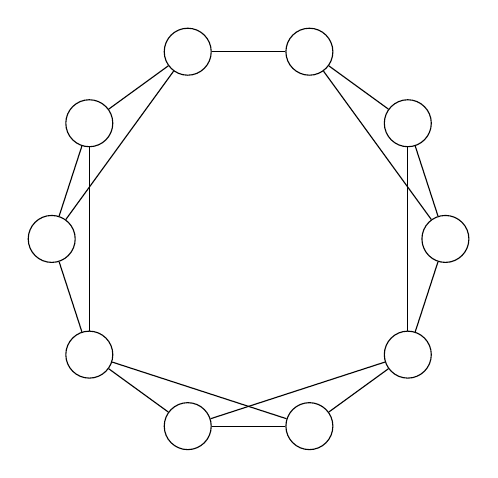
\begin{tikzpicture}

            \newcount \c
            \foreach \n in {0, ..., 9}{
                \c=\n
                \multiply\c by -36
                \advance\c by 90
                \advance\c by 18
                \node[draw, circle, inner sep=6pt, font=\large] (N\n) at (\the\c:2.5) {~};
            }

            \draw (N0) -- (N1);
            \draw (N1) -- (N2);
            \draw (N1) -- (N3);
            \draw (N2) -- (N3);
            \draw (N2) -- (N4);
            \draw (N3) -- (N4);
            \draw (N4) -- (N5);
            \draw (N4) -- (N6);
            \draw (N5) -- (N6);
            \draw (N5) -- (N7);
            \draw (N6) -- (N7);
            \draw (N7) -- (N8);
            \draw (N7) -- (N9);
            \draw (N8) -- (N0);
            \draw (N8) -- (N9);
            \draw (N9) -- (N0);

        \end{tikzpicture}
        \end{center}
    }

    \only<3>{
        \begin{center}
        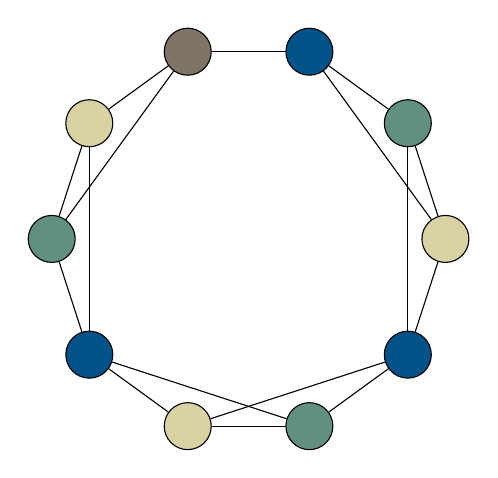
\begin{tikzpicture}

            \newcount \c
            \foreach \n in {0, ..., 9}{
                \c=\n
                \multiply\c by -36
                \advance\c by 90
                \advance\c by 18
                \ifthenelse{\n = 1 \OR \n = 4 \OR \n = 7} {
                    \node[draw, circle, inner sep=6pt, font=\large, fill=uofgblue] (N\n) at (\the\c:2.5) {~};
                }{}
                \ifthenelse{\n = 2 \OR \n = 5 \OR \n = 8} {
                    \node[draw, circle, inner sep=6pt, font=\large, fill=uofgtdarkgreen] (N\n) at (\the\c:2.5) {~};
                }{}
                \ifthenelse{\n = 3 \OR \n = 6 \OR \n = 9} {
                    \node[draw, circle, inner sep=6pt, font=\large, fill=uofgtyellow] (N\n) at (\the\c:2.5) {~};
                }{}
                \ifthenelse{\n = 0} {
                    \node[draw, circle, inner sep=6pt, font=\large, fill=uofgstone] (N\n) at (\the\c:2.5) {~};
                }{}
            }

            \draw (N0) -- (N1);
            \draw (N1) -- (N2);
            \draw (N1) -- (N3);
            \draw (N2) -- (N3);
            \draw (N2) -- (N4);
            \draw (N3) -- (N4);
            \draw (N4) -- (N5);
            \draw (N4) -- (N6);
            \draw (N5) -- (N6);
            \draw (N5) -- (N7);
            \draw (N6) -- (N7);
            \draw (N7) -- (N8);
            \draw (N7) -- (N9);
            \draw (N8) -- (N0);
            \draw (N8) -- (N9);
            \draw (N9) -- (N0);

        \end{tikzpicture}
        \end{center}
    }

    \only<4>{
        \begin{columns}[T]
            \column{.7\textwidth}
            \centering\includegraphics*[keepaspectratio=true,scale=0.18]{images/colouring-code.png}

            \column{.3\textwidth}
            \centering\includegraphics*[keepaspectratio=true,scale=0.18]{images/colouring-graph.png}
        \end{columns}
    }

    \only<5>{
        \begin{centering}
            \input{colouring/gen-simple}
        \end{centering}
    }

    \only<6>{
        \begin{centering}
            \input{colouring/gen-bigger}
        \end{centering}
    }

    \only<7>{
        \begin{centering}
            \input{colouring/gen-bigger59}
        \end{centering}
    }

    \only<8>{
        \begin{centering}
            \input{colouring/gen-bigger37}
        \end{centering}
    }
\end{frame}

\begin{frame}{Measuring Parallel Improvements}
    \only<1>{
        \begin{itemize}
            \item \emph{Speedup} is sequential runtime divided by parallel runtime.
                \begin{itemize}
                    \item Ideally, over a good sequential algorithm, not a parallel algorithm run with one
                        thread. This is sometimes called \emph{absolute} speedup.
                    \item This may not be practical if using special hardware.
                \end{itemize}

            \item A \emph{linear} speedup is a speedup of $n$ using $n$ processors.
                \begin{itemize}
                    \item This is not a realistic expectation on modern hardware.
                \end{itemize}
        \end{itemize}
    }

    \only<2>{
        \begin{itemize}
            \item \emph{Balance} is whether every compute unit is kept busy doing useful work.

            \item A \emph{regular} problem is one which can easily be split into equally sized units of
                work. Irregular problems are hard to balance.

            \item Often only a small number of the decision problems are ``really hard'', so we get poor
                balance.
        \end{itemize}
    }

    \only<3>{
        \begin{itemize}
            \item Most parallel algorithms contain a ``sequential'' part which cannot be parallelised,
                and a ``parallel'' part.

            \item \emph{Amdahl's law} says that if the sequential portion is fixed and we divide the
                parallel portion perfectly among $n$ processors, and if $k$ is the fraction of the
                work we cannot parallelise, then \[
                    \mathit{best~speedup} = \frac{1}{k + \frac{1}{n}\left(1 - k\right)}
                \]

            \item For CP algorithms, things get much more complicated, so it is important to understand
                where the formula comes from (using primary school maths), rather than memorising it.

            \item \emph{Gustafson's law} deals with using more processors to tackle larger problems.
        \end{itemize}
    }

    \only<4>{
        \begin{itemize}
            \item We need a large parallelisable portion of the algorithm, \emph{and} good work
                balance, or we don't get much of an improvement.
        \end{itemize}
    }
\end{frame}

\begin{frame}{Fixed Parallel Tree Search?}

    \begin{center}
        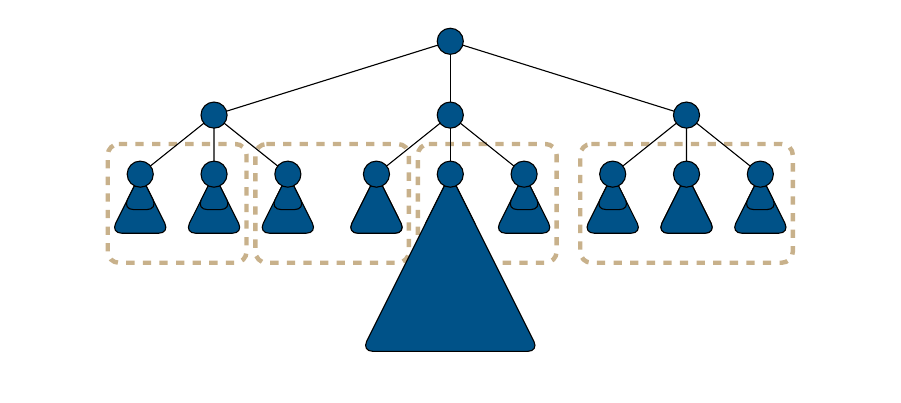
\begin{tikzpicture}[scale=0.75]%{{{
        \coordinate (R);

        \coordinate (N) at (R);

        \coordinate (N1) at ($(N) + (-4, -1.25)$);
        \coordinate (N2) at ($(N) + ( 0, -1.25)$);
        \coordinate (N3) at ($(N) + ( 4, -1.25)$);

        \foreach \na in {1, ..., 3}{
            \coordinate (N\na 1) at ($(N\na) + (-1.25, -1)$);
            \coordinate (N\na 2) at ($(N\na) + ( 0,    -1)$);
            \coordinate (N\na 3) at ($(N\na) + ( 1.25, -1)$);

            \foreach \nb in {1, ..., 3}{
                \coordinate (N\na\nb t1) at ($(N\na\nb) + (-0.5, -1)$);
                \coordinate (N\na\nb t2) at ($(N\na\nb) + ( 0.5, -1)$);

                \coordinate (N\na\nb s1) at ($(N\na\nb) + (-0.3, -0.6)$);
                \coordinate (N\na\nb s2) at ($(N\na\nb) + ( 0.3, -0.6)$);

                \coordinate (N\na\nb h1) at ($(N\na\nb) + (-1.5, -3)$);
                \coordinate (N\na\nb h2) at ($(N\na\nb) + ( 1.5, -3)$);
            }
        }

        \tikzstyle{p} = [draw, rounded corners, dashed, color=uofgtorange, ultra thick];
        \draw <2-3> [p] ($(N11) + (-0.55, 0.51)$) -- ($(N12) + (0.55, 0.51)$) -- ($(N12) + (0.55, -1.5)$) -- ($(N11) + (-0.55, -1.5)$) -- cycle;
        \draw <2-3> [p] ($(N13) + (-0.55, 0.51)$) -- ($(N21) + (0.55, 0.51)$) -- ($(N21) + (0.55, -1.5)$) -- ($(N13) + (-0.55, -1.5)$) -- cycle;
        \draw <2-3> [p] ($(N22) + (-0.55, 0.51)$) -- ($(N23) + (0.55, 0.51)$) -- ($(N23) + (0.55, -1.5)$) -- ($(N22) + (-0.55, -1.5)$) -- cycle;
        \draw <2-3> [p] ($(N31) + (-0.55, 0.51)$) -- ($(N33) + (0.55, 0.51)$) -- ($(N33) + (0.55, -1.5)$) -- ($(N31) + (-0.55, -1.5)$) -- cycle;

        \foreach \na in {1, ..., 3}{
            \draw (N) -- (N\na);
            \foreach \nb in {1, ..., 3}{
                \draw (N\na) -- (N\na\nb);
            }
        }

        \tikzstyle{t} = [draw, fill, fill=uofgblue, rounded corners];
        \foreach \na in {1, ..., 3}{
            \foreach \nb in {1, ..., 3}{
                \draw <1-2> [t] (N\na\nb) -- (N\na\nb t1) -- (N\na\nb t2) -- cycle;
            }
        }

        \draw <3> [t] (N11) -- (N11s1) -- (N11s2) -- cycle;
        \draw <3> [t] (N12) -- (N12s1) -- (N12s2) -- cycle;
        \draw <3> [t] (N13) -- (N13s1) -- (N13s2) -- cycle;

        \draw <3> [t] (N21) -- (N21t1) -- (N21t2) -- cycle;
        \draw <3> [t] (N22) -- (N22h1) -- (N22h2) -- cycle;
        \draw <3> [t] (N23) -- (N23s1) -- (N23s2) -- cycle;

        \draw <3> [t] (N31) -- (N31s1) -- (N31s2) -- cycle;
        \draw <3> [t] (N32) -- (N32t1) -- (N32t2) -- cycle;
        \draw <3> [t] (N33) -- (N33s1) -- (N33s2) -- cycle;

        \tikzstyle{c} = [draw, circle, fill, fill=uofgblue];
        \node [c] at (N) { };

        \foreach \na in {1, ..., 3}{
            \node [c] at (N\na) { };

            \foreach \nb in {1, ..., 3}{
                \node [c] at (N\na\nb) { };
            }
        }

        \node at (-7, -5.5) { }; \node at (7, -5.5) { };
    \end{tikzpicture}%}}}
    \end{center}
\end{frame}

\begin{frame}{Parallel Portfolios?}
    \begin{itemize}
        \item Irregularity seems to be a problem\ldots How about a different approach? We may have
            many choices available:

            \begin{itemize}
                \item Models
                \item Heuristics
                \item Search algorithms
                \item Levels of consistency
                \item Solvers
            \end{itemize}

        \item What if we try lots of different combinations in parallel?

        \item Now our runtimes are determined by whoever finishes first, not whoever finishes last.
    \end{itemize}
\end{frame}

\begin{frame}{Parallel Consistency?}
    \only<1>{
        \begin{columns}[T]
            \column{.5\textwidth}
            \centering\includegraphics*[keepaspectratio=true,scale=0.12]{images/disac4-paper.png}

            \column{.5\textwidth}
            \centering\includegraphics*[keepaspectratio=true,scale=0.12]{images/disac4-linear.png}
            \vspace{0.5em}
            \centering\includegraphics*[keepaspectratio=true,scale=0.12]{images/disac4-massive.png}
        \end{columns}

        \vspace{3em}

        \begin{columns}[T]
            \column{.5\textwidth}
            \centering\includegraphics*[keepaspectratio=true,scale=0.12]{images/parallel-consistency-paper.png}

            \column{.5\textwidth}
            \centering\includegraphics*[keepaspectratio=true,scale=0.12]{images/parallel-consistency-method.png}
            \vspace{1em}
            \centering\includegraphics*[keepaspectratio=true,scale=0.12]{images/parallel-consistency-results.png}

        \end{columns}
    }

    \only<2>{
            \centering\includegraphics*[keepaspectratio=true,scale=0.25]{images/parallel-consistency-method.png}
    }

    \only<3>{
        \begin{center}\includegraphics*[keepaspectratio=true,scale=0.25]{images/disac4-linear.png}\end{center}

        \vspace{2em}

        \begin{center}\includegraphics*[keepaspectratio=true,scale=0.25]{images/parallel-consistency-results.png}\end{center}
    }

    \only<4>{
        \centering\includegraphics*[keepaspectratio=true,scale=0.25]{images/disac4-massive.png}
    }

    \only<5>{
        \centering\includegraphics*[keepaspectratio=true,scale=0.1]{images/acpc-paper.png}

        \vspace{2em}

        \centering\includegraphics*[keepaspectratio=true,scale=0.1]{images/acpc-abstract.png}

        \vspace{2em}

        \centering\includegraphics*[keepaspectratio=true,scale=0.1]{images/acpc-practical.png}

        \vspace{0em}
    }

    \only<6>{
        \centering\includegraphics*[keepaspectratio=true,scale=0.2]{images/acpc-abstract.png}

        \vspace{0em}
    }

    \only<7>{
        \centering\includegraphics*[keepaspectratio=true,scale=0.2]{images/acpc-practical.png}

        \vspace{0em}
    }
\end{frame}

\begin{frame}{A Little Bit of Heresy}
    \only<1>{
        \centering\includegraphics*[keepaspectratio=true,scale=0.4]{images/acpc-poly.png}

        \vspace{0em}
    }

    \only<2>{
        \centering\includegraphics*[keepaspectratio=true,scale=0.4]{images/cheese.jpg}

        \vspace{0em}

        \begin{center}
            ``I want to buy a polynomial number of processors.''
        \end{center}
    }

    \only<3>{
        \centering\includegraphics*[keepaspectratio=true,scale=0.4]{images/xeon.png}

        \vspace{0em}
    }

    \only<4>{
        \centering\includegraphics*[keepaspectratio=true,scale=0.4]{images/archer-spec.png}

        \vspace{0em}
    }

    \only<5>{
        \centering\includegraphics*[keepaspectratio=true,scale=0.2]{images/constants.png}

        \vspace{0em}
    }

    \only<6>{
        \centering\includegraphics*[keepaspectratio=true,scale=0.5]{images/inquisition.jpg}

        \vspace{0em}
    }
\end{frame}

\begin{frame}{Representing Domains}
    \begin{itemize}
        \item A variable's domain contains a set of values.
        \item How should we implement this this?
            \begin{itemize}
                \item \visible<2>{A list.}
                \item \visible<2>{An array.}
                \item \visible<2>{A tree.}
                \item \visible<2>{A purely functional tree.}
                \item \visible<2>{A hash set.}
                \item \visible<2>{Just a pair of values, if we're doing bounds consistency.}
                \item \visible<2>{\ldots}
            \end{itemize}
    \end{itemize}
\end{frame}

\begin{frame}{Bitsets and Bit Parallelism}
    \only<1>{
        \begin{itemize}
            \item Domains are sometimes small and compact.

            \item If domains have no more than 64 values, we can store them in (long unsigned) integers.
                We have one bit per value. $0$ means ``not in the set'' and $1$ means ``in the set''.

            \item We can use arrays of integers for larger domains. (And we can go up to 512 bit
                integers on some Intel CPUs.)
        \end{itemize}
    }

    \only<2>{
        \begin{itemize}
            \item This is hardware-friendly: the entire model might fit in cache. Pushing and
                popping world takes a few nanoseconds.

            \item Setting a domain to take exactly one value: \[
                    d \gets 1 \ll v
                \]

            \item Testing whether or not a value is present in a domain: \[
                    d~\&~(1 \ll v) \ne 0
                \]

            \item Turning a single bit off: \[
                    d \gets d~\&~\text{\textasciitilde}(1 \ll v)
                \]

            \item There are dedicated hardware instructions for all of these in recent CPUs. We can
                also count the number of set bits (how many values are left in our domain?), and
                find the first set bit (pick a value from the domain) in hardware.
        \end{itemize}
    }

    \only<3>{
        \begin{itemize}
            \item Some constraints are similarly bitset friendly.

            \item Extensional constraints (a list of all ``allowed pairs'') can be represented as
                a ``compatibility'' bitset for each value in each variable's domain. Now
                forward checking is just a bitwise ``and'' operation.
                \begin{itemize}
                    \item Uses a lot of memory, but if our model is reasonably small and dense
                        that's fine.
                \end{itemize}

            \item Less than, greater than, and certain arithmetic constraints.
                \begin{itemize}
                    \item Fun exercise: figure this out.
                \end{itemize}

            \item Some constraints are probably not bitset friendly.
        \end{itemize}
    }
\end{frame}

\begin{frame}[b]
    \vfill
    \begin{center}
    \url{http://dcs.gla.ac.uk/~ciaran} \\
    \href{mailto:c.mccreesh.1@research.gla.ac.uk}{\nolinkurl{c.mccreesh.1@research.gla.ac.uk}}
\end{center}
\begin{tikzpicture}[remember picture, overlay]
    \node at (current page.north west) {\begin{tikzpicture}[remember picture, overlay]\fill
    [fill=uofgblue, anchor=north west] (0, 0) rectangle (\paperwidth, -1.5cm);\end{tikzpicture}};
    \node [anchor=north west, shift={(0.2cm,-0.2cm)}] at (current page.north west) {\includegraphics*[keepaspectratio=true,scale=0.5]{UoG_keyline.eps}};
\end{tikzpicture}
\end{frame}

\end{document}


